% sample text
\chapter{Result and Analysis}\label{ch:result-and-analysis}


\section{Experimental Setup}\label{sec:experimental-setup}
The following table~\ref{tab:experiment_setup} describe computer specifications used in the experiment.
\begin{table}[htbp]
    \centering
    \caption{Experiment Setup with PC Specifications}
    \label{tab:experiment_setup}
    \begin{tabular}{|c|c|}
        \hline
        \textbf{PC Specifications}        & \textbf{Details}        \\
        \hline
        \multirow{2}{*}{Processor}        & Intel Core i7 8700K     \\
        & 6 cores / 12 threads    \\
        \hline
        RAM                              & 32GB                    \\
        \hline
        \multirow{2}{*}{Graphics Card}    & NVIDIA GeForce GTX 1070 \\
        & 8GB VRAM                \\
        \hline
        \multirow{2}{*}{Operating System} & Ubuntu 22.10            \\
        & Linux 5.13              \\
        \hline
        \multirow{2}{*}{Python Version}   & Python 3.7              \\
        & Anaconda distribution   \\
        \hline
    \end{tabular}
\end{table}

\paragraph In this section, we conducted experiments that compare
our PPO-Beta and standard PPO-Gaussian implementation.
We used MetaDrive~\cite{li2021metadrive} for traffic simulator~\cref{fig:metadrive-fig} which
support both single agent and multi-agent training with
integrated reinforcement learning interface (Gym)~\cite{brockman2016openai}. We
proposed 3 evaluation metrics such as training rewards, safety
rate, and success rate. Training reward is the feedback given
by the simulator as the score. When the agent drives and reach
the destination, 130 score (total reward) is given but we can
set the solving threshold as 80 as average solving score as it
implies that the agent already passes through the intersection
safely. For safety and success rate, they are collected in
evaluation stage which we loaded the pretrained model into
the agent as they are in real situation and let the agent run
without updating the policy. The success is the ratio of how
many times the agent reaches the destination over the number
of agents participating in the evaluation. Safety is the ratio of
the agents successfully driving on the road without crashes to
other objects or vehicles. We run the traning for both algorithms for 5 tryouts and plot the average for each evaluation metric. The PPO hyperparameters are shown in table~\ref{tab:ppo_hyperparameters}.
\begin{table}[htbp]
    \centering
    \caption{PPO Configuration}
    \label{tab:ppo_hyperparameters}
    \begin{tabular}{|l|c|c|}
        \hline
        \textbf{PPO Method}  & \textbf{Beta (Ours)} & \textbf{Gaussian} \\
        \hline
        Clipping             & 0.02                 & 0.02              \\
        Gamma                & 0.99                 & 0.99              \\
        Action decay rate    & N/A                  & 0.005             \\
        Action initial Std   & N/A                  & 0.6               \\
        Minimum decay        & N/A                  & 0.1               \\
        K Epoch              & 5                    & 5                 \\
        Actor learning rate  & 0.0003               & 0.0003            \\
        Critic learning rate & 0.001                & 0.001             \\
        \hline
    \end{tabular}
\end{table}

Here is the explanation of the hyperparameters: Clipping is the clipping value for the PPO loss function.
Gamma is the discount factor for the reward.
Action decay rate is the decay rate for the action standard deviation.
Action initial Std is the initial standard deviation for the action.
Minimum decay is the minimum decay rate for the action standard deviation.
K Epoch is the number of epochs for the PPO update.
Actor learning rate is the learning rate for the actor network.
Critic learning rate is the learning rate for the critic network.
\section{Reward Shaping}\label{sec:reward-shaping}
We designed the reward funtion $R$ as:
\begin{equation}
    R = c_{1}(d_{t} - d_{t-1}) + c_{2}\frac{v_{t}}{v_{max}} + R_{T}
\end{equation}
where $d_{t}$ is the distance between the agent and the destination at time $t$, $v_{t}$ is the speed of the agent at time $t$, $v_{max}$ is the maximum speed of the agent, $R_{T}$ is the termination reward, and $c_{1}$ and $c_{2}$ are the coefficients for the distance and speed reward respectively.
We set $c_{1} = 1$ and $c_{2} = 1$.
The design is to encourage the agent to drive faster and reach the destination as soon as possible.
$R_{T}$ is the termination reward which can be one of the following:
\begin{itemize}
    \item $R_{T} = 10$ if the agent reaches the destination.
    \item $R_{T} = -5$ if the agent drives out of the road.
    \item $R_{T} = -5$ if the agent collides with other vehicles.
    \item $R_{T} = -5$ if the agent collides with other objects.
\end{itemize}


\section{Single Agent Result}\label{sec:single-agent-result}
\begin{figure}[H]
    \centering
    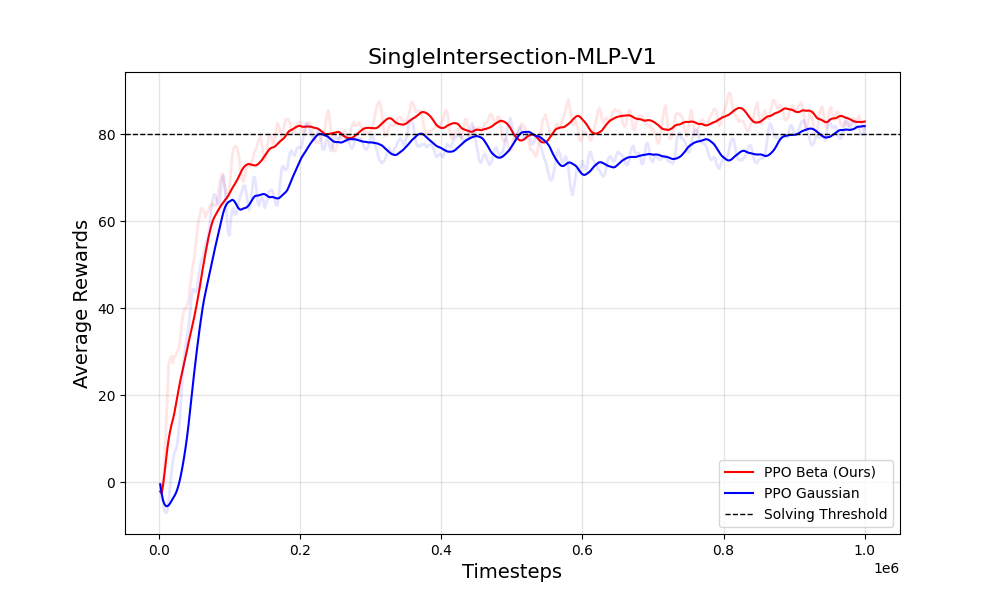
\includegraphics[width=14cm]{assets/ppo_single}
    \caption{Comparision of single agent traning}\label{fig:single_agent_training_reward}
    \medskip
    \small Comparison by average reward between PPO Beta (proposed method) and standard PPO Gaussian.
    The training is run for 1 million steps. We can see that PPO Beta has higher reward than standard PPO Gaussian which reach the solving threshold (80) faster.
    The training performance is also more stable than standard PPO Gaussian.
\end{figure}
\paragraph The Gaussian distribution implemented in standard PPO
has an adjustment nature that can lead to a drop in training
performance after the update of the value function as we can see in ~\cref{fig:single_agent_training_reward}. This is
because the Gaussian distribution is centered around the
mean, and when the mean is updated, the distribution must
shift to accommodate the new mean.
This shift can cause a
temporary drop in performance as the agent adjusts to the new
distribution. The Beta distribution, on the other hand, does not
suffer from this problem. The Beta distribution is more
flexible than the Gaussian distribution, and it can
accommodate changes in the mean without causing a
significant drop in performance. This is because the Beta
distribution is not centered around a single point, but rather it
is spread out over a range of values. This makes it more robust
to changes in the mean.
\begin{figure}[H]
    \centering
    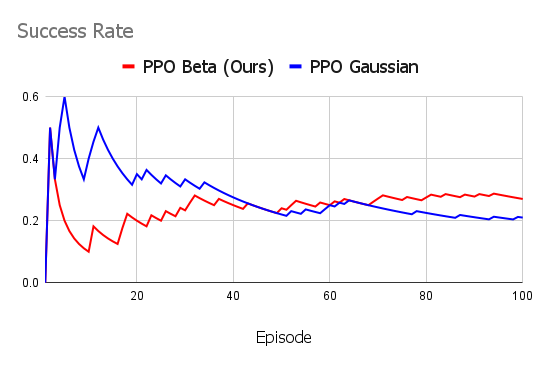
\includegraphics[width=9cm]{assets/single_success}
    \caption{Comparision of single agent traning by average success rate}\label{fig:single_agent_success_rate}
    \medskip
    \small We ran the evaluation for 100 episodes.
    We can see that PPO Beta has higher success rate than standard PPO Gaussian.
\end{figure}
In our experiments, we found that the Beta policy learned
to reach the solving threshold (80) faster than the Gaussian
policy. Additionally, the average score of the PPO-Beta agent
was slightly better than the PPO-Gaussian agent. These results
suggest that the Beta distribution is a more effective choice for
continuous control tasks than the Gaussian distribution.
\begin{figure}[H]
    \centering
    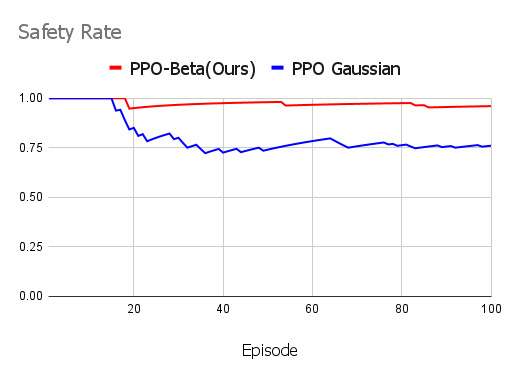
\includegraphics[width=9cm]{assets/single_safety}
    \caption{Comparision of single agent traning by average safety rate}\label{fig:figure6}
    \medskip
    \small We ran the evaluation for 100 episodes.
    We can see that PPO Beta has higher safety rate than standard PPO Gaussian.
\end{figure}
We evaluated the performance of PPO-Beta and PPO-Gaussian in a single-agent environment where the training
agent had difficulty predicting the actions of the other agents,
which were controlled by non-player characters (NPCs). We
found that PPO-Beta outperformed PPO-Gaussian on both the
success and safety rates after running for 100 episodes. As
shown in~\cref{fig:figure6}, both success rates were below 50\%.
This is because the single-agent environment is inherently difficult,
as the training agent cannot coordinate its actions with the
other agents.
Despite the difficulty of the environment, PPO-Beta was able to learn to dodge the incoming vehicle better
than PPO-Gaussian. This is evident in the safety rate, which
was 10\% higher for PPO-Beta than for PPO-Gaussian. These
results suggest that PPO-Beta is a more effective choice for
single-agent environments where the training agent has
difficulty predicting the actions of other agents.


\section{Multi Agent Result}\label{sec:multi-agent-result}
\begin{figure}[H]
    \centering
    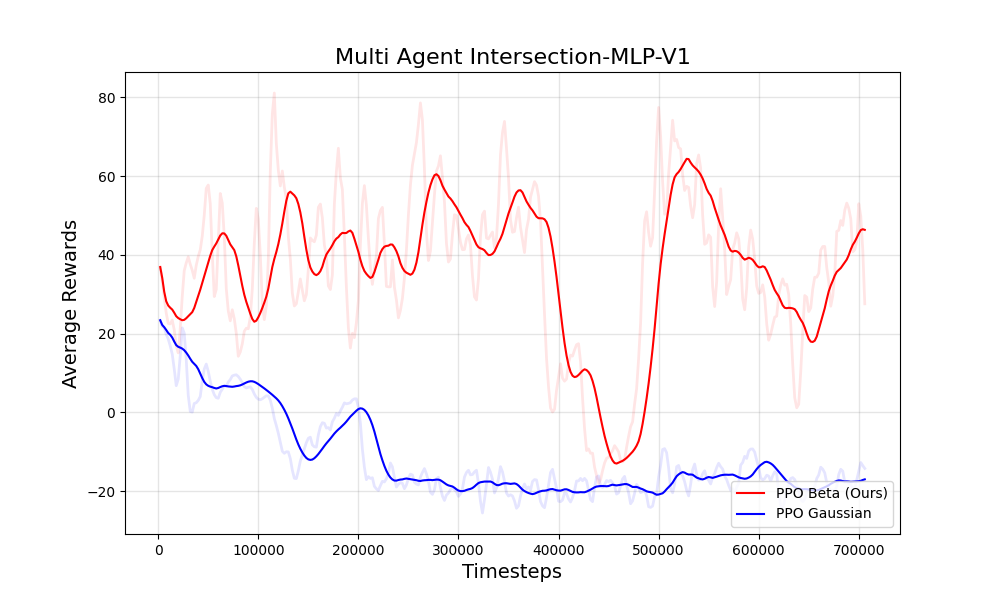
\includegraphics[width=14cm]{assets/multi-reward}
    \caption{Comparision of multi-agent traning by average reward}\label{fig:figure7}
    \medskip
    \small Comparison by average reward of 4 agents between PPO Beta (proposed method) and standard PPO Gaussian. The training is run for 700k steps. PPO with Gaussian distribution struggles to learn the environment and the reward is unstable.
\end{figure}

\paragraph We train the multi-agent environment with 4 agents.
Here is the interpretation of the result in \cref{fig:figure7}.
\subsection{Multi-agent PPO Beta}\label{subsec:multi-agent-ppo-beta}
\begin{itemize}
    \item \textbf{Average Reward:} The average reward obtained by the agents over all episodes is approximately 120. This indicates that, on average, the agents perform reasonably well in the environment when using the PPO beta approach.
    \item \textbf{Reward Fluctuations:} The rewards fluctuate throughout the training process. This fluctuation might be caused by various factors, such as the complexity of the environment, the number of agents interacting, and the training dynamics of PPO beta. It is normal to observe some variance in rewards during training.
    \item \textbf{Learning Stability:} The training curve does not show any significant spikes or crashes, which suggests that the training process using PPO beta is stable.
\end{itemize}
\subsection{Multi-agent PPO with Gaussian Distribution}\label{subsec:multi-agent-ppo-with-gaussian-distribution}
\begin{itemize}
    \item \textbf{Average Reward:} The average reward is lower compared to the multi-agent PPO beta. It indicates that using the Gaussian distribution approach might not be as effective in achieving high rewards as the PPO beta in this specific environment.
    \item \textbf{Reward Fluctuations:} Similar to PPO beta, the rewards fluctuate, but it seems to have higher variance with this approach. It is possible that the Gaussian distribution has a higher sensitivity to certain parameters or initial conditions.
    \item \textbf{Learning Stability:} As with PPO beta, there are no apparent stability issues with this approach.
\end{itemize}
Overall, from this data, it seems that the multi-agent PPO beta performs better in this particular environment compared to the multi-agent PPO with Gaussian distribution.
It is worth noting that RL experiments can be sensitive to hyperparameters and initial conditions, so it is essential to perform multiple runs with different seeds to assess the robustness of the results. In this case, we run each experiment with 5 tryouts and plot the average reward over all runs. This helps to reduce the variance in the results and provides a more accurate representation of the performance of each approach.

